\pgfdeclarelayer{background}
\pgfsetlayers{background,main}

\def\network{{(1.5, 2)/a}, {(2,2.7)/b}, {(4,2)/c}, {(5,2)/d}, {(5,1)/e}, {(4.5,0.5)/f}, {(3.5,0.5)/h}, {(3.5, -0.5)/i}, {(2.5, -0.5)/j}, {(1.5, -0.5)/k}, {(1,-0.5)/l}, {(1, 0.5)/m}}
\def\baseConnect{s/a, a/b, b/*, t/c, c/d, d/e, e/f, f/h, h/i, i/j, j/k, k/l, l/m, m/s}

\tikzstyle{vertex}=[circle,fill=black!25,minimum size=10pt,inner sep=0pt]
\tikzstyle{invis-vertex}=[circle,fill=white!100,minimum size=0pt, inner sep=0pt]
\tikzstyle{edge} = [draw,thick,-]
\tikzstyle{weight} = [font=\small]

\tikzstyle{selected edge} = [draw,line width=5pt,-,gray!50]
\tikzstyle{invis-vertex}=[circle,fill=white!100,minimum size=0pt, inner sep=0pt]

\colorlet{circle edge}{black!50}
\tikzset{
  outline/.style={draw=circle edge, thick}
  }

\subfloat[Initial]{\label{fig:short_path1}
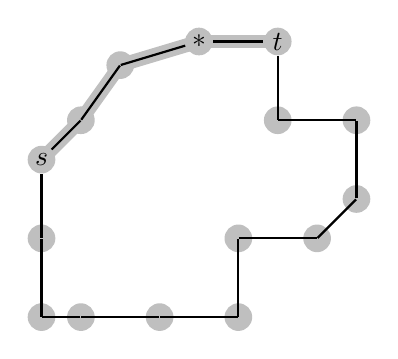
\begin{tikzpicture}
  % We draw the source and the sink, and the node that moves around
  \foreach \pos/\name in {{(1,1.5)/s}, {(4,3)/t}, {(3, 3)/*}} { 
    \node[invis-vertex] (\name-) at \pos {};
    \node[vertex] (\name) at \pos {$\name$};
  }
    
  % First we draw the rest of the vertices
  \foreach \pos/\name in \network {
    \node[invis-vertex] (\name) at \pos {};
    \node[vertex] () at \pos {};
  }
   
  % Connect vertices with edges and draw weights
  \foreach \source/ \dest in \baseConnect
    \path[edge] (\source) -- (\dest);
    
  \foreach \source/ \dest in {*/t}
    \path[edge] (\source) -- (\dest);
    
  \begin{pgfonlayer}{background}
    \foreach \source/ \dest in {s-/a, a/b, b/*-, *-/t-}
      \path[selected edge] (\source) -- (\dest);
  \end{pgfonlayer}
\end{tikzpicture}}
% Remove empty line
\subfloat[Node $*$ has moved]{\label{fig:short_path2}
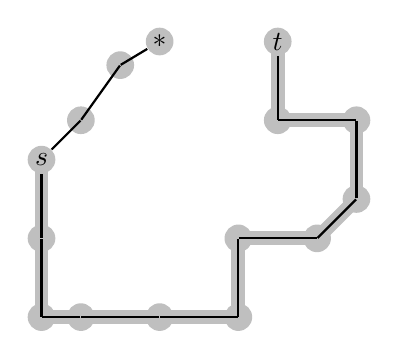
\begin{tikzpicture}
  % We draw the source and the sink
  \foreach \pos/\name in {{(1,1.5)/s}, {(4,3)/t}, {(2.5, 3)/*}} {
    \node[invis-vertex] (\name-) at \pos {};    
    \node[vertex] (\name) at \pos {$\name$};
  }
  % First we draw the vertices
  \foreach \pos/\name in \network {
    \node[invis-vertex] (\name) at \pos {};
    \node[vertex] () at \pos {};
  }

  % Connect vertices with edges and draw weights
  \foreach \source/ \dest in \baseConnect
    \path[edge] (\source) -- (\dest);

  \begin{pgfonlayer}{background}
    \foreach \source/ \dest in {s-/m, m/l, l/k, k/j, j/i, i/h, h/f, f/e, e/d, d/c, c/t-}
      \path[selected edge] (\source) -- (\dest);
  \end{pgfonlayer}
\end{tikzpicture}}
